%--------------------------------------------------------------------------------
%
% Text příspěvku do sborníku EEICT
%
% Vytvořil:  Martin Hruska
% Datum:     17.2.2013
% E-mail:    xhrusk16@stud.fit.vutbr.cz
%
%--------------------------------------------------------------------------------
%
% Přeložení: pdflatex prispevek.tex
%
% Optimální způsob použití = přepište jen vlastní text
%
\documentclass{eeict}
\inputencoding{utf8}
\usepackage{comment}
\usepackage{amsmath}
\usepackage{epstopdf}
\usepackage[bf]{caption2}
\usepackage{hyperref}
%--------------------------------------------------------------------------------

\title{Efficient Algorithms for Finite Automata}
\author{Martin Hruška}
\programme{Bachelor Degree Programme (3), FIT BUT}
\emails{xhrusk16@stud.fit.vutbr.cz}

\supervisor{Ondřej Lengál}
\emailv{ilengal@fit.vutbr.cz}

\abstract{
Nondeterministic finite automata (NFA) are used in many areas of computer science, including, but not limited to, formal verification, or the design of digital
circuits. Their advantages over deterministic finite automata (DFA) is that they may be exponentially conciser. However, this advantage may be lost if a na\"{\i}ve
approach to some operations, in particular checking language inclusion, which performs explicit determinization of the NFA, is taken. Recently, several new
techniques for this problem that avoid explicit determinization (using the so-called antichains or bisimulation up to congruence) have been proposed. 
The main goal of this paper is to describe these techniques which are being implemented as the new extension for the VATA library.
%The main goal
%of this work is an efficient implementation of these techniques in the context of the VATA library.
}
\keywords{finite automata, formal verification, language inclusion, bisimulation up to congruence, antichains, simulation}

\begin{document}
% -- Hlavička práce --

\maketitle

%-------------------------------------------------------------------------------
\selectlanguage{english}
\section{Introduction}
A~finite automaton (FA) is a computation model with applications in different branches of computer science, e.g., compiler design, formal verification or 
the design of digital circuits. %or natural language processing. 
In formal verification alone are its uses abundant, 
e.g., in model checking of safety temporal properties, abstract regular model checking \cite{tacas10}, static analysis, 
or decision procedures of some logics, such as Presburger arithmetic or weak 
monadic second-order theory of one successor (WS1S) \cite{libvata}.

Many of the mentioned applications need to perform certain expensive operations on FA, such as checking universality of an FA (i.e., checking whether it
accepts any word over a given alphabet), or checking language inclusion of a pair of FA (i.e., testing whether the language of one FA is a subset of the language
of the second FA). The classical (so called \emph{textbook}) approach is based on complementation of the language of an FA \cite{cav06}. 
Complementation is easy for 
\emph{deterministic} FA (DFA)---just swapping accepting and non-accepting states---but a hard problem for \emph{nondeterministic} FA (NFA), which need 
to be determinized first (this may lead to an exponential explosion in the number of the states of the automaton). 
Both mentioned operations over NFA are PSPACE-complete problems \cite{cav06}.

Recently, there has been a considerable advance in techniques for dealing with these problems. The new techniques are either based on the so-called 
\emph{antichains} \cite{cav06,tacas10} or the so-called \emph{bisimulation up to congruence} \cite{popl13}. 
In general, those techniques do not need an explicit construction of the complement
automaton. They only construct a sub-automaton which is sufficient for either proving that the universality or inclusion hold, or finding a counterexample.

Unfortunately, there is currently no efficient implementation of a general NFA library that would use the state-of-the-art algorithms for the mentioned
operations on automata. The
closest implementation is VATA \cite{libvata}, a general library for nondeterministic finite \emph{tree} automata, which can be used even for NFA (being modelled 
as unary tree automata) but not with the optimal performance given by its overhead that comes with the ability to handle much richer structures. 

The goal of this work is two-fold: (i) extending VATA with an NFA module implementing basic operations on NFA, such as union, intersection, or 
checking language inclusion, and (ii) an efficient design and implementation of checking language inclusion of NFA using 
bisimulation up to congruence (which is missing in VATA for tree automata).

% 5x zmena \omega na w
\section{Preliminaries}
We call a finite set of symbols $\Sigma$ an \emph{alphabet}. A~\emph{word} $w$ over $\Sigma$ of \emph{length} $n$ is a finite sequence of symbols 
$w=a_1\ldots a_n$, where $\forall 1 \leq i \leq n\,.\,a_i \in \Sigma$. 
A~\emph{nondeterministic finite automaton} (NFA) is a quintuple $\mathcal{A}= (Q,\Sigma,\delta,I,F)$, 
where $Q$ is a finite set of states, $\Sigma$ is an alphabet, $\delta \subseteq Q\times \Sigma \times Q$
is a transition relation (we use $p \xrightarrow{a} q$ to denote that $(p,a,q) \in \delta$), $I \subseteq Q$ is a set of initial states 
and $F \subseteq Q$ is a set of final states. A~\emph{deterministic finite automaton} (DFA) is a special case of an NFA, 
where $\delta$ is a partial function 
$\delta: Q\times \Sigma \to Q$ and $|I| \leq 1$. A~\emph{run} of an NFA $\mathcal{A}=(Q,\Sigma,\delta,I,F)$ from a state $q$
over a word $w=a_1\ldots a_n$ is a sequence $r = q_0 \ldots q_n$, where $\forall 0\leq i \leq n\ .\ q_i\in Q$ 
such that $q_0=q$ and $(q_i,a_{i+1},q_{i+1})\in \delta$. 
The run $r$ is called \emph{accepting} iff $q_n \in F$. The~\emph{language} of state $q \in Q$ is defined as 
$L_\mathcal{A}(q) = \{w\in \Sigma^{*}\ |\ \emph{there exists an accepting run of }\mathcal{A} 
\emph{ from }q\emph{ over }w\}$, while the language of a set of states $R\subseteq Q$ is defined as $L_{\mathcal{A}}(R)=\bigcup_{q\in R}L_{\mathcal{A}}(q)$.
The language of an NFA $\mathcal{A}$ is defined as $L_{\mathcal{A}}=L_{\mathcal{A}}(I)$.

\section{Checking language inclusion of NFA}
Given a pair of automata $\mathcal{A}=(Q_1,\Sigma,\delta_1,I_1,F_1)$ and $\mathcal{B}=(Q_2,\Sigma,\delta_2,I_2,F_2)$,
the \emph{textbook} algorithm for checking inclusion of their languages $L_\mathcal{A}\subseteq L_\mathcal{B}$ works by first 
determinizing $\mathcal{B}$ (yielding the DFA 
$\mathcal{B}_{det}$), 
complementing it ($\overline{\mathcal{B}_{det}}$) and constructing the NFA $\mathcal{A} \times \overline{\mathcal{B}_{det}}$ 
accepting the intersection of $L_{\mathcal{A}}$ and ${L_{\overline{\mathcal{B}_{det}}}}$ and
checking whether its language is nonempty. Any accepting run in this automaton may serve as a witness that the inclusion between $\mathcal{A}$ 
and $\mathcal{B}$ does not hold. 
Some recently introduced approaches avoid the explicit construction of $\overline{\mathcal{B}_{det}}$ and the related state explosion in many cases.

\subsection{Antichains}
We define an antichain and simulation before describing the algorithm itself. 
Given a partially ordered set $Y$, an \emph {antichain} is a set $X \subseteq Y$ such that all elements of $X$ are incomparable.
A~forward \emph{simulation} on the NFA $\mathcal{A}$ is a relation $\preceq\  \subseteq Q_1 \times Q_1$ 
such that if $p \preceq r$ then (i) $p \in F_1 
\Rightarrow r \in F_1$ and (ii) for every transition $p\xrightarrow{a}p'$, there exists a transition 
$r\xrightarrow{a}r'$ such that $p' \preceq r'$. Note that simulation implies language inclusion, i.e., $p\preceq q \Rightarrow L_\mathcal{A}(p)
\subseteq L_\mathcal{A}(q)$.

The antichains algorithm \cite{cav06} starts searching for a final state of the automaton $\mathcal{A}\times \overline{\mathcal{B}_{det}}$ while
pruning out the states which are not necessary to explore. $\mathcal{A}$ is explored nondeterministically and $\mathcal{B}$ 
is gradually determinized, so the algorithm explores pairs $(p,P)$ where $p\in Q_1$ and $P\subseteq Q_2$. 
%Forward antichains algorithm starts building the product automaton from its start states (backward version starts from final states),
%derives new states along the product automaton transitions and inserts them to the set of visited pairs $X$. 
The antichains algorithm derives new states along the product automaton transitions and inserts them to the set of visited pairs $X$.
$X$ keeps only minimal elements with respect to the ordering given by $(r,R)\sqsubseteq (p,P)$ iff $r=p \wedge R \subseteq P$. 
If there is generated a pair $(p,P)$ and there is 
$(r,R)\in X$ such that $(r,R) \sqsubseteq (p,P)$, we can skip $(p,P)$ and not insert it to $X$ for further search.
 
An improvement of the antichains algorithm using simulation \cite{tacas10} is based on the following optimization. 
We can stop the search from a pair $(p,P)$ if either (a) there exists some already visited pair $(r,R)$ 
such that $p\preceq r \wedge \forall r'\in R\, \exists\, p' \in P: r' \preceq p'$, or (b) there is $p' \in P$ such that $p \preceq p'$.

\subsection{Bisimulation up to congruence}
Another approach to checking language inclusion of NFA is based on bisimulation up to congruence. This technique was originally developed for
checking equivalence of languages of automata but it can
also be used for checking language inclusion, based on the observation that $L_\mathcal{A}\cup L_\mathcal{B}= L_\mathcal{B} 
\Leftrightarrow L_\mathcal{A}\subseteq L_\mathcal{B}$. 
This approach is based on the computation of a~\emph{congruence closure} $c(R)$ 
for some binary relation on states of the determinized automaton $R \subseteq 2^Q\times 2^Q$ defined 
%associative, commutative, idempotent binary operation $+: Q\times Q \to Q$ 
as a relation $c(R)=(r\cup s\cup t \cup u\cup id)^{\omega}(R)$, where $id(R)=R$, 
$r(R)=\{(X,X)\ |\ X\subseteq Q\}$, 
$s(R)=\{(Y,X)\ |\ XRY\}$,\linebreak
$t(R)=\{(X,Z)\ |\ \exists\,Y\subseteq Q,\ XRYRZ\}$,
$u(R)=\{(X_1 \cup X_2,Y_1\cup Y_2)\ |\ X_1 R Y_1 \wedge X_2 R Y_2\}$. 

The congruence algorithm works on a similar principle as the antichains algorithm. 
It starts building $\mathcal{A}_{det}$ and $\mathcal{B}_{det}$ and checks if macrostates in generated pairs are both
final or not. The optimization used is based on computing congruence closure of the set of already visited pairs of macrostates. 
If the generated pair is in this congruence closure, it can be skipped and further not processed.

Comparing the mentioned approaches to the checking language inclusion can be seen in Figure \ref{automata}.
\begin{figure}[bht]
\begin{center}
	\scalebox{1}
	{
		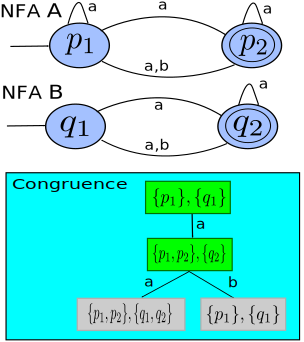
\includegraphics[scale=0.45]{congr1.eps}
		\hspace{0.55cm}
  	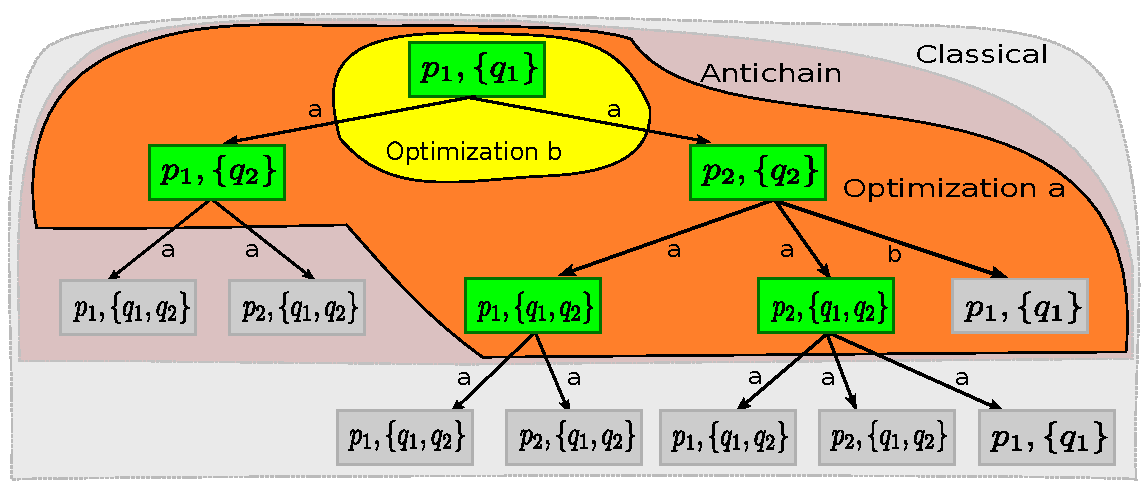
\includegraphics[scale=0.55]{ac1.eps}
	}
  \caption{
      \rm{
      \hspace{0.1cm} The picture is based on an example from \cite{tacas10}.
      It shows the procedure of checking language inclusion between two NFA using the mentioned approaches (which correspond to the labeled areas).
      %The labeled areas correspond to mentioned approaches.
      The antichain algorithm reduces number of the generated states compared with the classical,
      e.g., $(p_2,\{q_1,q_2\})$ is not further explored because $(p_2,\{q_2\}) \sqsubseteq (p_2,\{q_1,q_2\})$. 
      The optimization a and b are improvements of the antichain algorithm using simulation. 
      The congruence algorithm also reduces number of the generated states, so $(\{p_1,p_2\},\{q_1,q_2\})$ 
      is not further explored because it is in congruence closure 
      of the set of visited states.}}
      %It shows macrostates 
			%that are generated when checking language inclusion between two NFA using different approaches. Optimization a and b
			%correspond to the parts of the improvement of antichain algorithm using simulation.}}
  \label{automata}
\end{center}
\end{figure}


\section{Conclusion}
This paper briefly describes new approaches to checking language inclusion of NFA. These algorithms are being implemented in the new extension for
finite automata manipulation of VATA library.

\begin{comment}
\subsection{Obrázek}

%------------
% Příklad vložení obrázku do dokumentu.
\begin{figure}[bht]
\begin{center}
  \includegraphics[width=6cm,keepaspectratio]{bozka_ss}
  \caption{
      \rm{
      \hspace{0.1cm} Obrázek Božetěchovy.}}
  \label{bozka_ss.jpg}
\end{center}
\end{figure}
\end{comment}

%%% ZALOHA PRELIMINARIES
\begin{comment}
\section{Preliminaries}
We call a finite set of symbols $\Sigma$ an \emph{alphabet}. A~\emph{word} $w$ over $\Sigma$ of \emph{length} $n$ is a finite sequence of symbols 
$w=a_1\ldots a_n$, where $\forall 1 \leq i \leq n\ . \ a_i \in \Sigma$. An \emph{empty word} is denoted as $\epsilon \not\in\Sigma$ and its length is $0$. 
We define \emph{concatenation} as an associative binary operation on words over $\Sigma$ represented by the symbol $.$ such that for two words $u=a_1\ldots a_2$
and $v=b_1\ldots b_n$ over $\Sigma$ it holds that $\epsilon .u=u.\epsilon=u$ and $u.v=a_1 \ldots a_nb_1 \ldots b_m$. We define a symbol $\Sigma^{*}$ as set of all 
words over $\Sigma$ including the empty word and a symbol $Sigma^{+}$ as set of all words over $\Sigma$ without empty word. A~\emph{language} $L$ over $\Sigma$ is 
subset of $\Sigma^{*}$.

A~\emph{nondeterministic finite automata} is a quintuple $N= (Q,\Sigma,\delta,I,F)$, where $Q$ is set of all states of automaton, $\Sigma$ is alphabet, $\delta$
is called transition function and is defined as $\delta \subseteq Q\times \Sigma Q$. $I \subseteq Q$ is set of initial states 
and $F \subseteq Q$ is set of finite states. A~\emph{deterministic finite automata} is special case, where $\delta$ is a partial transition function defined as
$\delta: Q\times \Sigma \longrightarrow Q$ and $|I| \leq 1$. A~\emph{run} of a (non)deterministic automaton $M=(Q,\Sigma,\delta,I,F)$ 
over a word $w=a_1\ldots a_n$ is a sequence $r = q_0 \ldots q_n \in Q$ of states such that $q_0\in I$ and $(q_i,a_{i+1},q_{i+1})\in \delta$ 
for all $i: 0\leq i < n$. Run is called \emph{accepting}, iff $q_n \in F$. A~\emph{language accepted by (non)deterministic automaton} $M=(Q,\Sigma,\delta,I,F)$ 
is denoted as $L(M)$ and defined as $L(M) = \{w\in \Sigma^{*}\ |\ \emph{there exists accepting run of }$M$ \emph{ over }w\}$.
\emph{Language inclusion} of language of a (non)deterministic finite automaton $A$ with language of a (non)deterministic 
finite automaton $B$ is defined as $L(A)\cap\overline{L(B)} = \emptyset$.
Product of finite automaton $M_1=(Q_1,\Sigma,\delta,I_1,F)$ and finite automaton $M_2=(Q_2,\Sigma,\delta,I_2,F)$ 
is finite automaton $M_3=(Q_1 \times Q_2,\Sigma,\delta,I_1\times I_2,F_1\times F_2)$, where $\delta = \{((q_1,q_2),a,(q_1',q_2'))\ |\ (q_1,a,q_1') \wedge 
(q_2,a,q_2')\}$, where $a\in\Sigma$.
Now let define how to construct equivalent DFA $M_{det}$ for a given NFA $M=(Q,\Sigma,\delta,S,F)$. This textbook 
approach is called \emph{subset construction} and defines determinized automaton as $M_{det}=(2^Q,\Sigma,\delta_{det},S,F_{det})$, where $2^Q$ is power set of $Q$,
$F_{det}=\{Q'\subseteq Q\ |\ Q'\cap F \not = \emptyset\}$, $\delta_{det}(Q',a)=\bigcup_{q\in Q'}\delta(q,a)$, where $a\in\Sigma$.

 
Let $S$ be a \emph{partially order} set. Two elements $a,b\in S$ are incomparable iff $neither\ a \leq b, nor\ b \leq a$.
An \emph{antichain} is a set $A \subseteq S$, where $A \subseteq S~=\{\forall a,b \in A\ .\ a\not\in b \cap b \not a\}$.
A~forward \emph{simulation} on NFA $A=(Q,\Sigma,\delta,I,F)$ is a relation $\preceq\  \subseteq Q \times Q$ such that $p \preceq r$ iff (i) $p \in F 
\Rightarrow r \in F$ and (ii) for every transition $p \xrightarrow{a} p'$, there exists a transition $r \xrightarrow{a} r'$ such that $p' \preceq r'$ 
Let $X$ be a set with n-ary operation $O$ over $X$. 
Let have two NFA $A=(Q_1,\Sigma,\delta,I_1,F_1)$ and $B=(Q_2,\Sigma,\delta,I_2,F_2)$ and relation $R \subseteq 2^{Q_1} \times 2^{Q_2}$. A~\emph{congruence closure}
of relation $R$ is relation $c(R)=(r\cup s~\cup t \cup u~\cup id)^{w}(R)$, where $id$ is identity on $R$, 
$r(R)=\{(x,x)\ |\ \forall x\in 2^{Q_1} \times 2^{Q_2}\}$, $s(R)=\{(y,x)\ |\ xRy\}$, 
$t(R)=\{(x,z)\ |\ \exists y,\ xRyRz\}$, $u(R)=\{(x_1+x_2,y_1+y_2)\ |\ x_1 R x_2 \cap y_1 R y_2\}$.
\emph{Congruence} is an equivalence relation $R$, which follows this condition 
$\forall a_1,\ldots,a_n,b_1,\ldots,b_n\in X$:	$a_1 \sim_{R} b_1,\ldots,a_n \sim_{R} b_n \Rightarrow O_n(a_1,\ldots,a_n) \sim_{R} O_n(b_1,\ldots,b_n)$.
The finite iterations of a function $f: X\rightarrow X$ are denoted by $f^{n}$, where $f^{0}(x)=x$ and $f^{n+1}=f(f^{n}(x))$. The omega iteration of 
function $f$ is defined by $f^{w}=\bigcup_{n\geq 0}f$.
\end{comment}

\begin{comment}
\subsection{Antichains algorithm}
Antichains algorithm also checks language inclusion over NFA 
with searching for an accepting state of product automaton $A\times \overline{B}$, but it
prunes out some states, which are unnecessary to explore. Automaton $A$ is explored nondeterministically and automaton $B$ deterministically so the product
automaton's states are pairs $\{(p,P) \ . \ p\in Q_1 \wedge P\in 2^{Q_2}\}$. 
%Forward antichains algorithm starts building the product automaton from its start states (backward version starts from final states),
%derives new states along the product automaton transitions and inserts them to the set of visited pairs $X$. 
The antichains algorithm builds the product automaton from its start states,
derives new states along the product automaton transitions and inserts them to the set of visited pairs $X$. 
On this set $X$ is defined ordering by $(r,R)\sqsubseteq (p,P)$, iff $r=p \wedge R \subseteq P$. 
If there is during construction of product automaton generated state $(p,P)$ and there is 
$(r,R)\in X$ such that $(r,R) \sqsubseteq (p,P)$, we can skip $(p,P)$ and do not give it to $X$. By intuition, we do not have to care about $p$ and $r$ because
they are identical. $P$ is larger then $R$ so all
states accepted by $R$ are also accepted by $P$ (and it does not hold vice versa) so $R$ has greater chance to be nonaccepting state in determinized DFA $B_{det}$.
%(and so $(p,P)$ has greater chance to be accepting in product automaton $A\times\overline{B}$).
Set $X$ could be called antichain because it contains only incomparable elements. Base of this algorithm was introduced in \cite{cav06}.

The simulation improvement \cite{tacas10} of the antichains algorithm is based on the follow optimization. 
We can stop search from product-state $(p,P)$, if there exists some visited product state $(r,R)$ 
such that $p\preceq r \wedge R\preceq^{\forall\exists}P$, or $\exists p'\in P: p \preceq p'$. First part of condition says that 
if $(p,P)$ takes automaton to the accepting state, $(r,R)$ will be taken to accepting state too, so we do not have search from $(p,P)$. Second part of condition
shows, that every accepting word of $p$ takes $P$ to accepting state too,\linebreak because $\exists p'\in P: p \preceq p'$.

\subsection{Bisimulation up to congruence}
The another approach to checking inclusion over NFA is based on bisimulation up to congruence. This approach is primary for checking language equivalence but it can
also be used for checking language inclusion, when you consider that $L(A)\cup L(B)= L(B) \Rightarrow L(A)\subseteq L(B)$. 
The congruence algorithm is based on similar principle as antichain algorithm. 
It starts determinization of $A$ and $B$ simultaneously and checks, if newly generated states are equivalent (if they are either
finale or not). Optimization is based on computing congruence closure on the set of generated pair of states. 
If the newly generate pair is in this congruence
closure, it could be skipped. 
\end{comment}



%------------
% Poděkování
%
\section*{Acknowledgement}
%I~would like to thank my supervisor Ondřej Lengál for his advises and constructive criticism during the work.
This work was supported by the Czech Science Foundation within the project No. P103/10/0306.
%------------
% Citace
%
\begin{thebibliography}{9}
  \bibitem{cav06} M. De Wulf, L. Doyen, T.A. Henzinger and J.-F. Raskin  Antichains: A
		New Algorithm for Checking Universality of Finite Automata. In Proc. of CAV 2006. Springer-Verlag (2006).

  \bibitem{tacas10} P.A. Abdulla, Y.-F. Chen, L. Holík, R. Mayr and
		T. Vojnar. When Simulation Meets Antichains: On Checking Language Inclusion of
		Nondeterministic Finite (Tree) Automata. In Proc. of TACAS 2010. Springer-Verlag (2010).

	\bibitem{popl13} F. Bonchi and D. Pous. Checking NFA Equivalence with Bisimulations up
		to Congruence. In Proc. of POPL 2013. ACM (2013).
	
	\bibitem{libvata} O. Lengál, J. Šimáček and T. Vojnar. VATA: A~Library for Efficient
		Manipulation of Non-deterministic Tree Automata. In Proc. of TACAS 2012. Springer-Verlag (2012).

  %\bibitem{static} S. Hallem, B. Chelf, Y. Xie and D. Engler. A System and
  %Language for Building System-specific, Static Analyses. PLDI 2002. ACM (2002).
  

\end{thebibliography}

\end{document}
